In this chapter, the methods used to investigate the problem statement are
presented. First, the choice of method is described briefly and motivated, this
section will also cover the databases used and why these were picked. Following
this section comes a section describing the benchmark problems, that is the
data set used and the corresponding queries. Finally the implementation details
of the tool used is described in more detail.

\section{Choice of method}\label{sec:choiceofmethod}
This section will cover first why the databases used for evaluation were
chosen, following this dataset used for evaluation is motivated and finally a
short description of the technologies used.

\subsection{Choice of databases}\label{sec:choiceofdatabases}
The two database chosen to be evaluated are PostgreSQL and MariaDB.
Both of these databases fulfill the following criteria:
\begin{enumerate}
\item Modern databases that see much use and development;
\item Open-source projects with code that anyone can read, modify and help develop;
\item And they implement state-of-the-art algorithms and methods.
\end{enumerate}

In addition to this PostgreSQL is the typical choice for academic evaluation.
All research papers mentioned in Chapter~\ref{chap:relatedwork} that have
implemented new algorithms or modified old ones have done so in PostgreSQL.
MariaDB on the other hand is compatible with MySQL making it a common
alternative for enterprises. The two databases should therefore cover the most
commonly used open-source databases for academia and enterprises.

Studying these two databases should cover how well a modern state-of-the-art
query optimizer performs. In addition, as mentioned in Section~\ref{sec:purpose}
since both of them are open-source, if one performs better than the other the
code can be studied to identify areas of improvement.

\subsection{Choice of dataset}
The dataset used for evaluation is one taken directly from the real-world, this
is to ensure that the database has all the traits of a real database:
non-trivial indexes, non-uniform and skewed data as well as a considerable
amount of data.

One important reason that the dataset was selected was that most of the ones
currently used for evaluation such as TPC-H, TPC-DS or more recently JOB (REFERENCE), all
have trivial index setups; that is one index on the primary key for each
relation. As such, studying how the query optimizer selects index for these is
irrelevant: there is just one index trivially found to be correct.

The relevant statistics of the dataset are shown in Section~\ref{sec:benchmark}

\subsection{Choice of technologies used}
The technologies used to develop the tool used for evaluation were chosen to be
Clojure, using a JDBC driver. The reason these were selected is that Clojure
runs on the JVM, making it platform independent. In addition most of the work
done by the tool is to process and transform data in the form of JSON, a task
that Clojure is well suited to.

\section{Benchmark problems}\label{sec:benchmark}
This section will give a description if the problems used for benchmarking the
query optimizers. The section will start with a description of the relevant
statistics of the data set, following that is a description of the queries
chosen to evaluate the query optimizer.

\subsection{Hardware used}
The hardware used for testing is a dedicated computer running only the databases
and nothing else. The configuration parameters for the database are those of a
standard setup for PostgreSQL and MariaDB respectively.

The exact specifications of the hardware are not relevant as the choice of index
selection does not depend on those, but rather the software of the database itself.

\subsection{The data set}
- number of tables, size of some tables, number of indexes etc

\subsection{The queries}
- focus on using tables with many indexes
- join several tables to improve errors and increase difficulty for the optimizer
- focus on using realistic queries actually used by trioptima to allow for
better and more realistic modeling

\section{Implementation}
This section will cover the implementation details of the tool, starting with
some of the technologies and frameworks used. Following this is a description of
the two steps of the analysis. Finally the queries used for PostgreSQL and
MariaDB respectively are presented.

The tool was implemented in Clojure, using JDBC to connect to and query the
databases. The tool is called via the command line and an example execution can
be seen in Figure~\ref{fig:cmd:running}. For more information regarding the
tool, see the public repository at GitHub.

\begin{figure}[ht]
  \caption[Running the tool from the command line]{An example of running the
  tool from the command line with some parameters.}
  \begin{lstlisting}[language=bash]
    lein run queries=query1 query2 repetitions=100 samplesizes=10 100 --database=postgresql
  \end{lstlisting}~\label{fig:cmd:running}
\end{figure}

The evaluation is split up into two separate processes:
\begin{enumerate}
\item Repeatedly executing queries with different sample sizes;
\item And then parsing the output of the executions to find the access methods used.
\end{enumerate}

The following sections will describe each of the two processes separately.

\subsection{Query execution}\label{sec:queryexecution}
During the query execution data is gathered about one or more queries, repeated
a number of times with a number of different sample sizes used. All resulting
query plans are then saved to a file for later parsing and evaluation.

The execution of one query consists of:
\begin{enumerate}
\item Delete all statistics gathered by the database if necessary;
\item Set the parameter that controls the sample size used;
\item Gather statistics about the tables used in the query;
\item Find the query plan chosen by the query optimizer for the given query;
\item And finally save the output to a file.
\end{enumerate}

This procedure is then repeated for each query and each sample size, a number of
times to find all possible query plans used. Pseudocode describing this process
can be found in Algorithm~\ref{fig:code:gathering}.

\begin{algorithm}
\caption[Pseudocode for the data gathering]{The algorithm used when
  gathering data about queries.}\label{fig:code:gathering}
\begin{algorithmic}[1]
  \For{each $query$ \Pisymbol{psy}{206} $queries$ }
    \For{each $samplesize$ \Pisymbol{psy}{206} $samplesizes$}
      \For{each $i$ \Pisymbol{psy}{206} $repitions$}
        \State delete statistics;
        \State set statistics target to $samplesize$
        \State analyze database tables
        \State analyze query
        \State add result to file
      \EndFor
    \EndFor
  \EndFor
\end{algorithmic}
\end{algorithm}

\subsection{Parsing and analyzing}\label{sec:parsing}
During the parsing and analysis a file generated from the previous process
(described in~\ref{sec:queryexecution}) is parsed and then analyzed to find what
access methods are used for each relation.

Analyzing one query consists of:
\begin{enumerate}
\item Identifying all relation accesses;
\item Grouping the relation accesses by what relation they access;
\item Finding all unique relation accesses per relation;
\item And finally calculating the size of the unique relation accesses per relation.
\end{enumerate}

This procedure is repeated for each repetition of each query and each sample
size. Pseudocode describing this process can be found in Algorithm~\ref{fig:code:analyzing}.

\begin{algorithm}
\caption[Pseudocode for the parsing and analyzing]{The algorithm used to analyze
the output of the query execution.}\label{fig:code:analyzing}
\begin{algorithmic}[1]
  \For{each $queryplan$ \Pisymbol{psy}{206} $queryplans$ }
    \State let relationaccesses = groupby(``relations'', findindexes(queryplan))
    \For{each $accessmethods$ \Pisymbol{psy}{206} $relationaccesses$}
      \State count(unique($accessmethods$))
    \EndFor
  \EndFor
\end{algorithmic}
\end{algorithm}

\subsection{PostgreSQL}
The commands used by PostgreSQL to delete the statistics gathered, set the
sample size and analyze the tables can be
seen in Figures~\ref{fig:sql:pgstatistics},~\ref{fig:sql:pgsamplesize} and
\ref{fig:sql:pganalyze} respectively.

\begin{figure}[ht]
\begin{lstlisting}[language=SQL]
  DELETE FROM pg_statistics;
\end{lstlisting}
\caption[Clearing the statistics in PostgreSQL]{The query used to clear out all
  statistics generated by ANALYZE in PostgreSQL.}
\label{fig:sql:pgstatistics}
\end{figure}

\begin{figure}[ht]
\begin{lstlisting}[language=SQL]
  SET default_statistics_target TO :SAMPLE_SIZE;
\end{lstlisting}
\caption[Setting the sample size in PostgreSQL.]{The query used to set the
  sample size used by PostgreSQL when gathering data via ANALYZE.}
\label{fig:sql:pgsamplesize}
\end{figure}

\begin{figure}[ht]
\begin{lstlisting}[language=SQL]
  ANALYZE table1;
  ANALYZE table2;
\end{lstlisting}
\caption[Analyzing the tables in PostgreSQL.]{The query used to make PostgreSQL
  gather statistics about all tables in the database.}
\label{fig:sql:pganalyze}
\end{figure}

\subsection{MariaDB}
The SQL queries used to test MariaDB can be seen in
Figures~\ref{fig:sql:mdbstatistics},~\ref{fig:sql:mdbsamplesize},~\ref{fig:sql:mdbanalyze}

\begin{figure}[ht]
\begin{lstlisting}[language=SQL]
  SET GLOBAL innodb_stats_persistent='OFF';
  SET GLOBAL innodb_stats_auto_recalt='OFF';
\end{lstlisting}
\caption[Ensure InnoDB use the stats we sample.]{The query used to ensure that
  InnoDB will use the stats we sample.}
\label{fig:sql:mdbstatistics}
\end{figure}

\begin{figure}[ht]
\begin{lstlisting}[language=SQL]
  SET GLOBAL innodb_stats_transient_sample_pages = :SAMPLE_SIZE;
\end{lstlisting}
\caption[Setting the sample size in MariaDB.]{The query used to set the sample
  size used by MariaDB when gathering data via ANALYZE.}
\label{fig:sql:mdbsamplesize}
\end{figure}

\begin{figure}[ht]
\begin{lstlisting}[language=SQL]
  ANALYZE TABLE table1, table2;
\end{lstlisting}
\caption[Analyzing the tables in MariaDB.]{The query used to make MariaDB
  gather statistics about the queried tables in the database.}
\label{fig:sql:mdbanalyze}
\end{figure}

\section{Evaluation}
Here are some the results found from the evaluation.

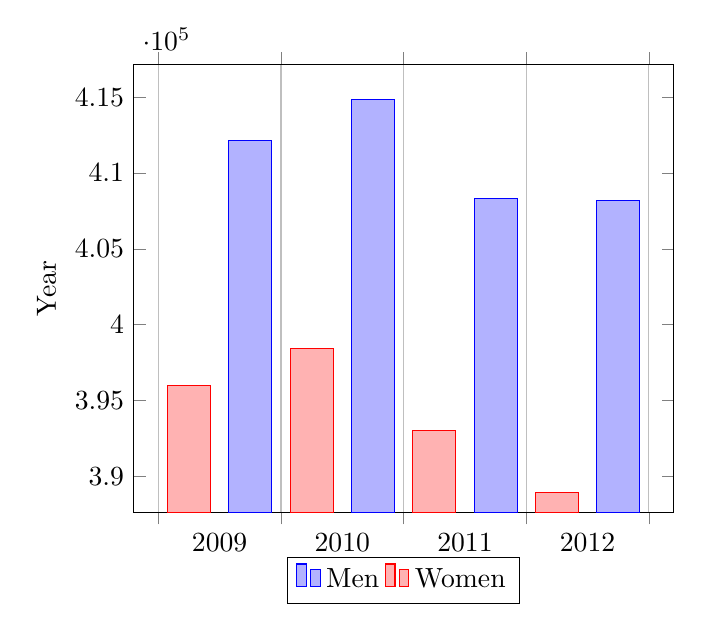
\begin{tikzpicture}
\begin{axis}[
	x tick label style={
		/pgf/number format/1000 sep=},
	ylabel=Year,
	enlargelimits=0.05,
	legend style={at={(0.5,-0.1)},
	anchor=north,legend columns=-1},
	ybar interval=0.7,
]
\addplot
	coordinates {(2012,408184) (2011,408348)
		 (2010,414870) (2009,412156) (2008,415 838)};
\addplot
	coordinates {(2012,388950) (2011,393007)
		(2010,398449) (2009,395972) (2008,398866)};
\legend{Men,Women}
\end{axis}
\end{tikzpicture}